\section{Comparison}
Using the PID Simulink box, four different controllers were developed to compare their behavior for the moving angle system. This comparison allowed to choose the adequate controller for the application of this project. Hence, the Figure \ref{fig:comp_pid} shows the four controllers tested.

\begin{figure}[H]
\centerline{
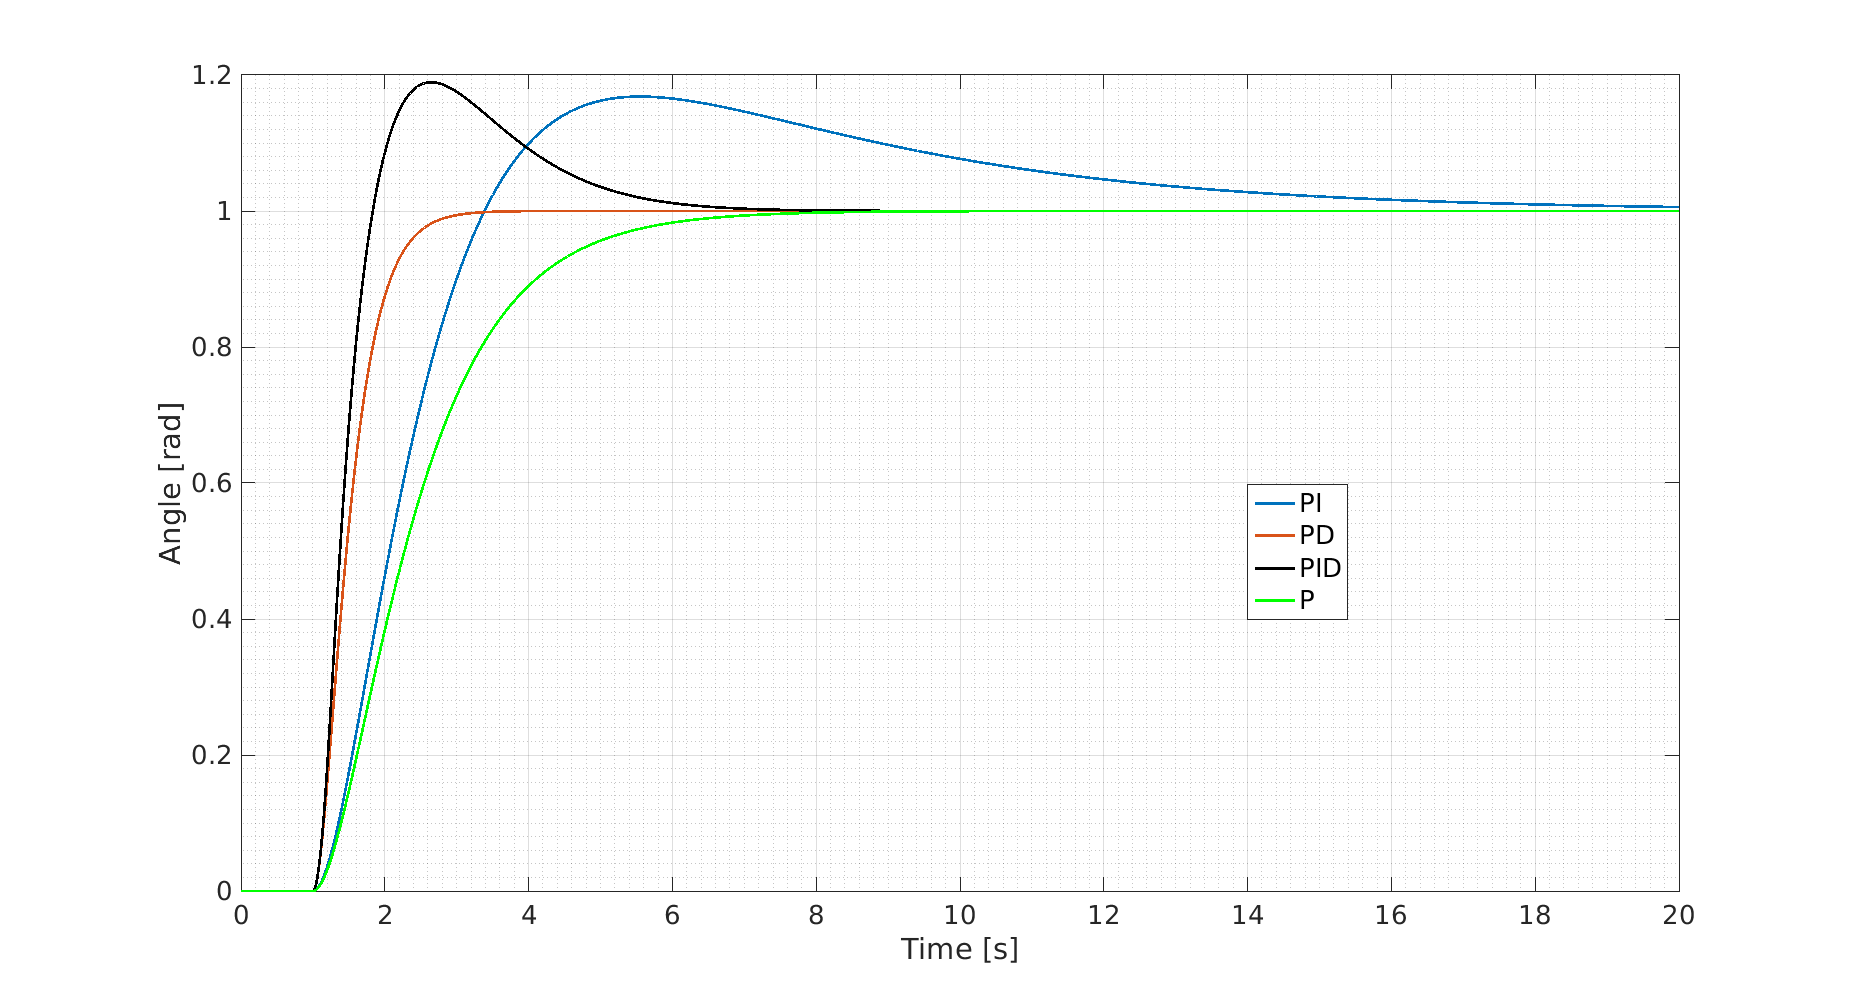
\includegraphics[scale=0.35]{figures/full_comp.png}}
\caption{Step response of the different controllers.}
\label{fig:comp_pid}
\end{figure}

The PI and the PID controllers are the ones with the highest overshoot due to their integral term. In point of fact, an important difference between the current and the desired value in the start of the simulation occurs, resulting in the growth of the integral part of the controller. 
Such overshoots (respectively, 0.19 and 0.16 radian for the PID and PI) are not viable for this application. Going over the desired angle, could result in loosing the connection between the UA and the GS.

Thus, the PD and P controllers were designed in order to avoid any overshoot. These controllers have a shorter settling time than the ones having an integral part. By having no overshoot and a fast response, the PD and the P controller are suitable for this project. The steady state error resulting from not including an integral component can not be avoid. However, its effect was tested in the Chapter \ref{ch:sim} and showed that it is not as significant.

\vspace{5mm}

Later, noise was added to the model of the moving angle system and the behavior of the two chosen controllers were analyzed. The performance of the PD and P controllers can be seen in the Figure \ref{fig:noise_PID}.

\begin{figure}[H]
\centerline{
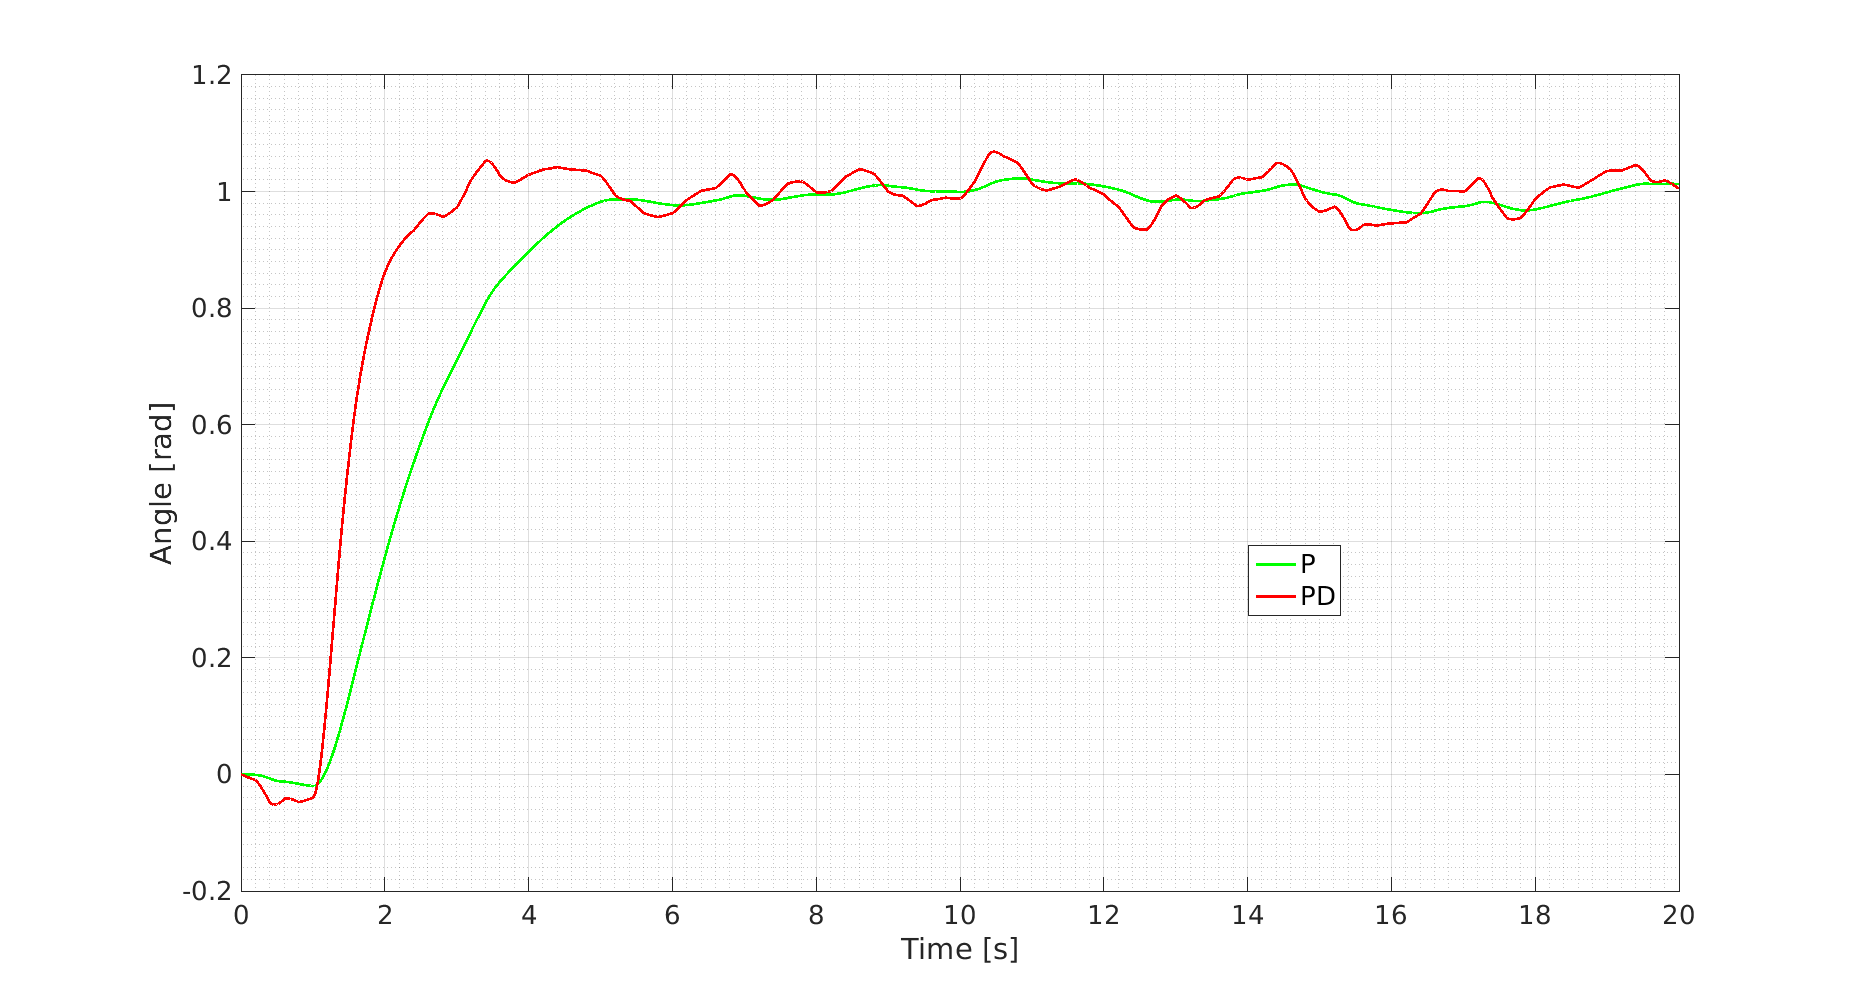
\includegraphics[scale=0.35]{figures/PD_noise.png}}
\caption{Effects of noise on the PD and P controllers.}
\label{fig:noise_PID}
\end{figure}

Both controllers present pros and cons. The PD controller is faster than the P one, but, on the other hand reacts more to noise. In the Chapter \ref{ch:sim} , these two controllers were tested to analyze the connection between the UA and the GS.